%
% 6-unschaerfe.tex
%
% (c) 2023 Prof Dr Andreas Müller
%
\section{Unschärfe-Relation
\label{buch:diskret:section:unschaerfe}}
Für die Fourier-Transformation auf der Gruppe $G=\mathbb{R}$ wurde die
Heisenberg-Pauli-Weyl-Un\-schärfe\-re\-la\-tion hergeleitet.
Sie besagt, dass eine Funktion und ihre Fourier-Transformierte nicht
gleichzeitig beliebig gut lokalisiert sein können.
Eine ähliche Eigenschaft gilt auch für Funktionen auf einer endlichen
Gruppe, sie ist der Inhalt des Satzes von Donoho-Stark
\cite{buch:donoho-stark}.
Das früher verwendete Lokalisierungsmass der Varianz lässt sich aber
nicht sinnvoll auf endliche Gruppen übertragen, daher beginnt die 
folgende Diskussion mit einer allgemeinen Diskussion von Lokalisierungsmassen.
Sie stützt sich auf das Paper \cite{buch:widgerson}.

%
% Lokalisierungsmasse
%
\subsection{Lokalisierungsmasse}
Für die Heisenberg-Pauli-Weyl-Unschärferelation verwendet die Varianz
als Mass für die Lokalisierung einer Funktion.
In diesem Abschnitt wird erst gezeigt, warum dieses Mass für Funktionen
auf endlichen Gruppen nicht funktioniert, danach wird ein alternatives
Lokalisierungsmass entwickelt.

\subsubsection{Varianz als Lokalisierungsmass in $\mathbb{R}$}
Zur Konstruktion eines Masses für die Lokalisierung einer Funktion
$f\colon \mathbb{R}\to\mathbb{C}$ wurde zunächst die nichtnegative
Funktion $\varphi(x) = \overline{f}(x)f(x) = |f(x)|^2$ gebildet,
die dann durch Normierung als Wahrscheinlichkeitsdichte interpretiert
wurde.
Die Varianz einer Zufallsvariable mit dieser Wahrscheinlichkeitsverteilung
$\varphi(x)$ ist dann ein mögliches Lokalisierungsmass.

Für die folgende Diskussion nehmen wir an, dass der Erwartungswert $0$
ist, dies lässt sich durch Translation der Funktion $f(x)$ immer erreichen.
Und auch für die Fourier-Transformierte $\hat{f}$ lässt sich dies
durch Multiplikation mit einem Phasenfaktor erreichen, der den
Erwartungswert von $f$ nicht ändert.

Die Normierung von $|f(x)|^2$ verwendet das Integral
\[
\int_{-\infty}^\infty \varphi(x) \,dx
=
\int_{-\infty}^\infty |f(x)|^2\,dx
=
\|f\|_2^2,
\]
also die $L^2$-Norm von $f(x)$.
Der Wert der Varianz ist damit
\[
H(f)
=
\int_{-\infty}^{\infty}
x^2
\frac{|f(x)|^2}{\|f\|_2^2} \,dx
=
\frac{1}{\|f\|_2^2}
\int_{-\infty}^{\infty} x^2\,|f(x)|^2\,dx.
\]
Dieses Unschärfemass lässt sich aber nicht auf periodische Funktionen
oder auf einen diskreten Definitionsbereich verallgemeinern.

Für periodische Funktionen bereitet bereits die Definition
des Erwartungswertes bereitet Schwierigkeiten.
Wenn $f(x)$ eine $2\pi$-periodische stetige Funktion ist, dann ist
\[
E(\delta)
=
\delta\mapsto 
\frac{1}{\|f\|_2^2}
\int_{-\pi+\delta}^{\pi+\delta}
x^2
|f(x)|^2
\,dx
\]
eine stetige Funktion mit der Eigenschaft $E(\delta+\pi)=E(\delta)+\pi$.
Der Wert $E(\delta)$ ist der Erwartungswert einer Zufallsvariablen
mit der Wahrscheinlichkeitsdichte $|f(x)|^2/\|f\|_2$ im Intervall
$[-\pi+\delta,\pi+\delta]$.
Es gibt also keinen einzelnen sinnvollen Wert für den Erwartungswert.

Für einen diskreten Definitionsbereich wird das Problem noch grösser.
Selbst wenn man sich auf ein Integrationsintervall festlegen könnte,
gäbe es Funktionen mit nicht ganzzahligem Erwartungswert.
Es muss also ein anderer Ansatz gefunden werden.

%
% Lokalisierung und Normen
%
\subsubsection{Lokalisierung und Normen}
Das Lokalisierungsmass soll anzeigen, in welchem Teil des Definitionsbereiches
die grösste ``Masse'' der Funktion gefunden werden kann.
Eine Funktion, deren Funktionswerte alle den gleichen Betrag
haben, hat keinen Argumentwert, der sinnvoll als ``Schwerpunkt''
angesehen werden könnte.

Auf der anderen Seite ist eine Funktion, die nur einen von $0$
verschiedenen Wert hat, ganz offensichtlich perfekt lokalisiert.
Die beiden Fälle können durch Vergleich geeigneter Normen 
unterschieden werden.
Sei also $f$ eine Funktion $G\to\mathbb{C}$ mit nur den einen von $0$
verschiedenen Wert $f(x_0)$ hat.
Die Supremumnorm
\[
\|f\|_\infty
=
\sup_{x\in G} |f(x)|
\]
von $f$ ist der maximale Wert $\|f\|_\infty = |f(x_0)|$.
Eine gar nicht lokalisierte Funktion $g\colon G\to\mathbb{C}$
mit der gleichen Supremumnorm hätte nur Werte mit Betrag
\[
|g(x)|
=
\|f\|_\infty\quad \forall x\in G.
\]
Ein grosser Unterschied zwischen $f$ und $g$ zeigt sich in
der $L^1$-Norm:
\begin{align*}
\|f\|_1
&=
\sum_{x\in G} |f(x)|
=
|f(x_0)|
=
\|f\|_\infty
&&\Rightarrow& \frac{\|f\|_1}{\|f\|_\infty}&=1
\\
\|g\|_1
&=
\sum_{x\in G} |g(x)|
=
|G|\cdot \|f\|_\infty
&&\Rightarrow& \frac{\|f\|_1}{\|f\|_\infty}&=|G|.
\end{align*}
Die nicht lokalisierte Funktion $f$ hat den minimal 
möglichen Wert $1$ und die lokalisierte Funktion $g$
hat den maximal möglichen Wert $|G|$.

\begin{definition}[Lokalisierungsmass]
\label{buch:diskret:unschaerfe:def:lokalisierungsmass}
Für eine Funktion $f\colon G\to\mathbb{C}$ ist das Lokalisierungsmass
\[
H(f)
=
\frac{\|f\|_1}{\|f\|_\infty}
=
\frac{\displaystyle\sum_{x\in G} |f(x)|}{\displaystyle\sup_{x\in G} |f(x)|}.
\]
\end{definition}

%
% Das allgemeine Unschärfeprinzip
%
\subsection{Das allgemeine Unschärfeprinzip}
Die Unschärferelation für die Fourier-Transformation vergleicht
die Lokalisierungsmasse der Funktionen $f$ und $\mathscr{F}f$.
Das allgemeine Unschärfeprinzip verallgemeinert dies auf eine
Aussage über beliebige lineare Abbildungen $A$.
Da das Lokalisierungsmass die Normen $\normfunc_1$ und $\normfunc_\infty$
miteinander vergleicht, muss untersucht werden, wie die Matrix $A$
diese Normen beeinflusst.

\begin{definition}[$U$-$V$-Norm]
\label{buch:diskret:unschaerfe:def:normUV}
Seien $U$ und $V$ zwei Vektorräume mit Normen $\normfunc_U$ und
$\normfunc_V$ und $A\colon U\to V$ eine lineare Abbildung.
Die Norm von $A$ ist
\begin{equation}
\|A\|_{U\to V}
=
\sup_{u\in U\setminus\{0\}} \frac{\| Au\|_V}{\|u\|_U}
\label{buch:diskret:unschaerfe:normUV}
\end{equation}
\end{definition}

Die Definition
\eqref{buch:diskret:unschaerfe:normUV}
der Norm bedeutet, dass
\[
\|Au\|_V \le \|A\|_{U\to V}\cdot \|u\|_U
\]
für alle $u\in U$.
Da auf den Vektorräumen, auf denen wir das Lokalisierungsmass
berechnen wollen verschiedene Normen definiert sein können,
müssen wir die Definition~\ref{buch:diskret:unschaerfe:def:normUV}.
noch etwas verallgemeinern.

\begin{definition}[Norm]
\label{buch:diskret:unschaerfe:def:norm1i}
Ist $A\colon U\to V$ eine lineare Abbildung und ist $\normfunc_p$
die $p$-Norm auf den Vektorräumen $U$ oder $V$, dann setzen wir
\[
\|A\|_{p\to q}
=
\sup_{u\in U\setminus\{0\}}
\frac{\|Au\|_q}{\|u\|_p}.
\]
\end{definition}

Mit diesen Voraussetzungen lässt sich jetzt das primäre Unschärfeprinzip
formulieren \cite{buch:widgerson}.

\begin{satz}[Das primäre Unschärfeprinzip]
\label{buch:diskret:unschaerfe:satz:primaer}
Sind $U$ und $V$ komplexe Vektorräume mit zwei Normen $\normfunc_\infty$
und $\normfunc_1$ und $A\colon U\to V$ und $B\colon V\to U$ lineare
Abbildungen mit $\|A\|_{1\to\infty}\le 1$ und $\|G\|_{1\to\infty}\le 1$.
Weiter sei angenommen, dass es eine Konstante $k>0$ gibt mit
$\|BAu\|_\infty \ge k\|u\|_\infty$.
Dann gilt für
\[
\|u\|_1\cdot \|Au\|_1 \ge k\|u\|_\infty\cdot \|Au\|_\infty
\]
alle $u\in U$.
\end{satz}

Die Bedingung für das Produkt $BA$ bedeutet, dass $BA$ invertierbar ist
und dass die Norm der inversen Abbildung
\[
\|(BA)^{-1}\|_{\infty\to\infty}
\ge k
\]
ist.
Insbesondere ist $A$ auch injektiv.

\begin{proof}[Beweis]
Aus $\|A\|_{1\to\infty}\le 1$ und $\|B\|_{1\to\infty}\le 1$ folgen
zunächst die Ungleichungen
\begin{align*}
\|Au\|_\infty &\le \|u\|_1
&&\text{und}&
\|BAu\|_\infty &\le \|Au\|_1.
\end{align*}
Für das Produkt gilt dann
\[
\|Au\|_\infty
\cdot
\|BAu\|_\infty
\le
\|u\|_1
\cdot
\|Au\|_1.
\]
Aus der Bedingung an das Produkt $BA$ kann die linke Seite nach unten
durch
\[
k\|u\|_\infty
\cdot
\|Au\|_\infty
\le
\|Au\|_\infty
\cdot
\|BAu\|_\infty
\le
\|u\|_1
\cdot
\|Au\|_1
\]
abgeschätzt werden.
Dies ist die behauptete Ungleichung.
\end{proof}

In Definition \ref{buch:diskret:unschaerfe:def:lokalisierungsmass}
wurde der Quotient von $L^1$-Norm und Supremumnorm als
Lokalsierungsmass definiert.
Damit kann das Unschärfeprinzip wie folgt umformuliert werden.

\begin{satz}[Unschärfe]
Unter den Voraussetzungen des
Satzes~\ref{buch:diskret:unschaerfe:satz:primaer}
gilt
\[
H(u)\cdot H(Au)
=
\frac{\|u\|_1}{\|u\|_\infty}
\cdot
\frac{\|Au\|_1}{\|Au\|_\infty}
\ge k
\]
für alle $u\in U\setminus\{0\}$.
\end{satz}

\begin{proof}[Beweis]
Die Behauptung folgt sofort aus Satz~\ref{buch:diskret:unschaerfe:satz:primaer}
durch Division durch $\|u\|_\infty\cdot \|Au\|_\infty$.
Allerdings ist noch zu verifizieren, dass der Faktor $\|Au\|_\infty$
nicht verschwinden kann.
Da aber aus der Voraussetzung an $BA$ folgt, dass $A$ injektiv ist
folgt aus $u\ne 0$, dass auch $Au\ne 0$ und damit $\|Au\|_\infty> 0$.
\end{proof}

%
% $k$-Hadamard-Matrizen
%
\subsection{$k$-Hadamard-Matrizen}
Die Bedingungen an das Produkt $BA$ in
Satz~\ref{buch:diskret:unschaerfe:satz:primaer}
motivieren die folgende Definition.

\begin{definition}[$k$-Hadamard-Matrix]
\label{buch:diskret:unschaerfe:def:khadamard}
Eine $n\times n$-Matrix heisst $k$-Hadamard wenn alle Einträge $a_{ik}$ von
\index{k-Hadamard-Matrix@$k$-Hadamard-Matrix}%
$A$ Betrag $|a_{ik}|\le 1$ haben und wenn
\begin{equation}
\|A^*Au\|_\infty \ge k\|u\|_\infty
\label{buch:diskret:unschaerfe:eqn:khadamard}
\end{equation}
gilt für alle $n$-dimensionalen Vektoren $u\in \mathbb{C}^n$.
\end{definition}

Die Bedingung 
\eqref{buch:diskret:unschaerfe:eqn:khadamard}
besagt, dass $A^*$ die Rolle der Matrix $B$ im primären
Unschärfeprinzip von Satz~\ref{buch:diskret:unschaerfe:satz:primaer}
einnehmen kann.

\begin{satz}[Unschärfe für $k$-Hadamard-Matrizen]
Ist $A$ eine $k$-Hadamard-Matrix dann gilt
\[
\|u\|_1\cdot \|Au\|_1 \ge k\|u\|_\infty \cdot \|Au\|_\infty
\]
für alle $u\in U$ oder
\[
H(u)\cdot H(Au)\ge k
\]
für alle $u \in U\setminus\{0\}$.
\end{satz}

Die Fourier-Transformation $\mathscr{F}_n$ ist eine $n\times n$-Matrix,
deren Einträge alle exakt den Betrag $1$ haben.
Ausserdem ist $\mathscr{F}_n^* = \overline{\mathscr{F}}_n$ und aus den 
bekannten Eigenschaften der Fourier-Transformation
\[
\mathscr{F}_n^*\mathscr{F}_n
=
\overline{\mathscr{F}}_n\mathscr{F}_n
=
nI
\qquad\Rightarrow\qquad
\| \mathscr{F}_n^*\mathscr{F}_n f\|_\infty
=
n \|f\|_\infty
\]
für alle $u\in\mathbb{C}^n$.
Die Fourier-Transformation $\mathscr{F}_n$ ist also eine
$n$-Hadamard Matrix.
Damit folgt jetzt der primäre Unschärfesatz für die Fourier-Transformation.

\begin{satz}[Unschärfe für diskrete Fourier-Transformation]
Für beliebige $f\in \mathbb{C}^n\setminus\{u\}$ gilt
\begin{equation}
H(u)\cdot H(\mathscr{F}_nu) \ge n.
\end{equation}
\end{satz}

%
% Träger als Lokalisierungsmass
%
\subsection{Träger als Lokalisierungsmass}
Das bisher verwendet Verhältnis $H(f)$ von $L^1$- und Supremumnorm
eines Vektors $f\in\mathbb{C}^n$ ist etwas aufwendig zu berechnen.
Ein einfacheres Mass ist die Anzahl der von $0$ verschiedenen
Funktionswerte.

%
% traeger.tex -- Traeger als Lokalisierungsmass
%
% (c) 2021 Prof Dr Andreas Müller, OST Ostschweizer Fachhochschule
%
\documentclass[tikz]{standalone}
\usepackage{amsmath}
\usepackage{times}
\usepackage{txfonts}
\usepackage{pgfplots}
\usepackage{csvsimple}
\usetikzlibrary{arrows,intersections,math}
\begin{document}
\def\skala{1}
\definecolor{darkgreen}{rgb}{0,0.6,0}
\begin{tikzpicture}[>=latex,thick,scale=\skala]

\fill[color=blue!20] (6,0) rectangle (11,6);

\draw[color=red] (0,6) --(13,6);
\node[color=red] at (3,6) [above] {$\|u\|_\infty$};

\draw[->] (-0.1,0) -- (13.5,0) coordinate[label={$x$}];
\draw[->] (0,-0.1) -- (0,6.5) coordinate[label={right:$y$}];

\node at (8,0) [below] {$T=\operatorname{supp}(u)$};

\draw[color=blue,line width=1.4pt] (6,0) -- (6,6) -- (11,6) -- (11,0);

\fill[color=darkgreen!40,opacity=0.5] 
	plot[domain=6:8,samples=100] ({\x},{3*(1-cos((\x-6)*(360/4)))})
	--
	plot[domain=8:11,samples=100] ({\x},{3*(1-cos((\x-5)*(360/6)))})
	-- cycle;

\draw[color=darkgreen,line width=1.4pt]
	(0,0)
	-- plot[domain=6:8,samples=100] ({\x},{3*(1-cos((\x-6)*(360/4)))})
	-- plot[domain=8:11,samples=100] ({\x},{3*(1-cos((\x-5)*(360/6)))})
	-- (13,0);

\node[color=darkgreen] at (8,2) {$\|u\|_1$};


\node[color=blue] at (6,3) [above,rotate=90] {$\|u\|_\infty\cdot\chi_T$};

\node[color=blue] at (11,6) [below left] {$\|u\|_\infty\cdot |T|$};

\end{tikzpicture}
\end{document}



Die Kardinalität des Trägers einer Funktion kann ebenfalls als
Lokalisierungsmass verwendet werden.
Je kleiner $|\operatorname{supp}f|$ ist, desto besser ist die
Funktion $f$ lokalisiert.

\begin{satz}[Unschärferelation für Träger]
\label{buch:diskret:unschaerfe:satz:supportsize}
Ist $A\in M_{n\times m}$ eine $k$-Hadamard-Matrix, dann gilt
\begin{equation}
|\operatorname{supp}u|
\cdot
|\operatorname{supp}Au|
\ge
k
\end{equation}
für jeden nichtverschwindenden Vektor $u\in\mathbb{C}^m$.
\end{satz}

\begin{proof}[Beweis]
Sei $u\ne 0$ und sei $\chi_{\operatorname{supp}u}$ die charakteristische
Funktion des Trägers $\operatorname{supp}u$, also
\[
\chi_{\operatorname{supp}u}(x)
=
\begin{cases}
1&\qquad\text{falls $x\in\operatorname{supp}(f)$ oder $f(x)\ne 0$}\\
0&\qquad\text{sonst.}
\end{cases}
\]
Dann ist
\[
|u(x)|
\le
\|f\|_\infty\cdot \chi_{\operatorname{supp}u}(x)
\quad
\text{für alle $x$.}
\]
Die Summe über den Definitionsbereich ergibt
\[
\|f\|_1
\le
\|f\|_\infty \|\chi_{\operatorname{supp}u}\|_1
=
\|f\|_\infty |\operatorname{supp}u|
\quad\Rightarrow\quad
\frac{\|u\|_1}{\|u\|_\infty} \le |\operatorname{supp}u|.
\]
Aus dem allgemeinen Unschärfeprinzip folgt
\[
k
\le
\frac{\|u\|_1}{\|u\|_\infty}
\cdot
\frac{\|Au\|_1}{\|Au\|_\infty}
\le
|\operatorname{supp}u|
\cdot
|\operatorname{supp}Au|.
\]
Dies beweist den Satz.
\end{proof}

\begin{satz}[Donoho-Stark]
\label{buch:diskret:unschaerfe:satz:donoho-stark}
\index{Donoho-Stark-Unschärfe}%
Für $f\colon G\to\mathbb{C}$ mit $f\ne 0$ gilt
\[
|\operatorname{supp}f|
\cdot
|\operatorname{supp}\mathscr{F}_nf|
\ge n.
\]
\end{satz}

\begin{proof}[Beweis]
Der Satz von Donoho-Stark folgt unmittelbar aus
Satz~\ref{buch:diskret:unschaerfe:satz:supportsize} und der
Tatsache, dass die Fourier-Transformation $\mathscr{F}_n$
$n=|G|$-Hadamard ist.
\end{proof}

%
% $\varepsilon$-Träger
%
\subsection{$(\varepsilon,p)$-Träger}
%
% etraeger.tex
%
% (c) 2023 Prof Dr Andreas Müller
%
\begin{figure}
\centering
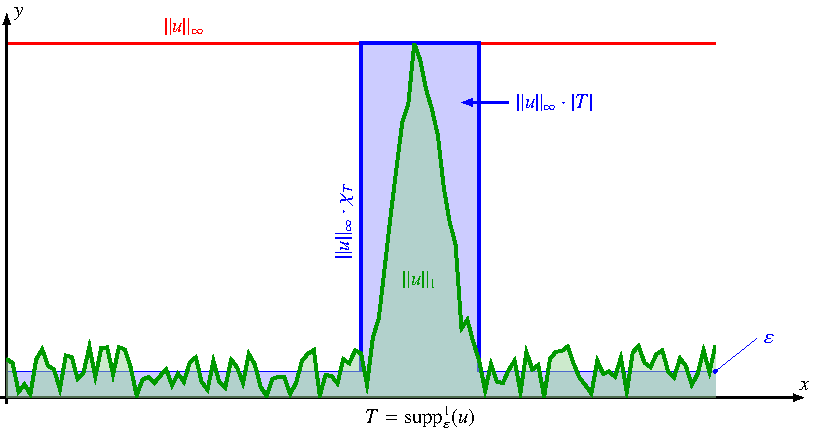
\includegraphics{chapters/060-diskret/images/etraeger.pdf}
\caption{$(\varepsilon,1)$-Träger als Mass für die Lokalsierung
einer Funktion.
Im Bereich der Menge $T$ ist die $L^1$-Norm des so gross, dass
die $L^1$-Norm auf dem Komplement von $L^1$ nur das $\varepsilon$-fache
der $L^1$-Norm $\|u\|_1$ ist.
\label{buch:diskret:unschaerfe:fig:etraeger}}
\end{figure}%

Rauschen sorgt dafür, dass man nicht erwarten kann dass ein
Signalvektor überhaupt Nullstellen hat.
Der Träger einer Funktionen ist also aus praktischen Grünen fast immer
der ganze Definitionsbereich.
Eine lokalisierte Funktion zeichnet sich also nicht mehr dadurch aus,
dass sie nur auf einer kleinen Menge von Punkten des Definitionsbereichs
grösser als eine gewählte untere Schranke $\varepsilon$ ist.
Dies führt auf die folgende Definition.

\begin{definition}[$(p,\varepsilon)$-Träger]
Man sagt die Menge $T$ ist ein {\em $(p,\varepsilon)$-Träger} eines Vektors
$u\in\mathbb{C}^n$, wenn 
\[
\| u\cdot (1-\chi_T)  \|_p \le \varepsilon \|u\|_p.
\]
\index{pepsilon-Träger@$(p,\varepsilon)$-Träger}%
\end{definition}

Da die Funktion $1-\chi_T$ in der Menge $T$ verschwindet und ausserhalb
den Wert $1$ hat, ist
$u\cdot (1-\chi_T)$ eine Funktion, in der alle Funktionswerte von
Argumenten in $T$ zu $0$ gemacht worden sind.
Die Norm $\| u\cdot (1-\chi_T) \|_p$ bewertet also nur den Anteil der
Funktion ausserhalb von $T$.
Die Bedingung an einen $(p,\varepsilon)$-Träger ist also die Forderung,
dass die Norm des Teils der Funktion ausserhalb $T$ höchstens das
$\varepsilon$-fache der Norm der ganzen Funktion ist.
Diese Situation ist in der Abbildung~\ref{buch:diskret:unschaerfe:fig:etraeger}
veranschaulicht.

\begin{definition}[$(p,\varepsilon)$-Trägergrösse]
Die $(p,\varepsilon)$-Trägergrösse ist
\[
|\operatorname{supp}_\varepsilon^p u|
=
\min \{ |T|\mid \text{$T$ ist eine $(p,\varepsilon)$-Träger von $u$}\}.
\]
\end{definition}

Da der Definitionsbereich endlich ist, gibt es auch nur endlich viele
Teilmengen $T$, die $(p,\varepsilon)$-Träger sein könnten.
Die Definition verlangt nicht, dass es nur einen einzigen kleinsten
$(p,\varepsilon)$-Träger gibt, es kann durchaus auch mehrere geben.
Trotzdem werden wir die Notation $\operatorname{supp}_\varepsilon^p u$
für einen dieser kleinsten $(p,\varepsilon)$-Träger zulassen.

In Anlehnung an den Satz~\ref{buch:diskret:unschaerfe:satz:donoho-stark}
möchten wir ein Unschärfe-Resultat für das Unschärfe-Mass
$|\operatorname{supp}_\varepsilon^1 u|$ herleiten.
Dazu ist es nötig, einen Zusammenhang zwischen
$|\operatorname{supp}_\varepsilon^1 u|$ und $H(u) = \|u\|_1/\|u\|_\infty$ 
herzustellen.
Sei also $T$ ein $(\varepsilon,1)$-Träger von $u$.
Dann ist
\[
u = u\cdot \chi_T + u\cdot (1-\chi_T).
\]
Die $L^1$-Norm ist
\[
\|u\|_1
=
\|u\cdot \chi_T\|_1
+
\|u\cdot (1-\chi_T)\|_1
\le
\|u\cdot \chi_T\|_1
+
\varepsilon \|u\|_1
\]
und nach Subtraktion des zweiten Terms auf der rechten Seite
\[
(1-\varepsilon)\|u\|_1 \le \|u\cdot\chi_T\|_1.
\]
Die rechte Seite kann wie im Beweis von
Satz~\ref{buch:diskret:unschaerfe:satz:donoho-stark}
durch die Supremumnorm abschätzen und ist
\[
\|u\cdot \chi_T\|_1 \le |T| \cdot \|u\|_\infty.
\]
Da dies für alle $(\varepsilon,1)$-Träger gilt, folgt
\begin{equation}
(1-\varepsilon) \|u\|_1
\le
|\operatorname{supp}_\varepsilon^1 u|\cdot \|u\|_\infty
\qquad
\Rightarrow
\qquad
\frac{\|u\|_1}{\|u\|_\infty}
\le
\frac{|\operatorname{supp}_\varepsilon^1 u|}{1-\varepsilon}.
\label{buch:diskret:unschaerfe:eqn:supp1}
\end{equation}
Damit folgt jetzt aus dem allgemeinen Unschärfeprinzip der folgende
Satz.

\begin{satz}[$\varepsilon$-$\delta$-Unschärfe für $k$-Hadamard-Matrix]
\index{epsilon-delta-Unschaerfe@$\varepsilon$-$\delta$-Unschärfe}%
Ist $A$ eine $k$-Hadamard-Matrix und $\varepsilon,\delta\in [0,1)$,
dann gilt
\[
|\operatorname{supp}_\varepsilon^1 u|
\cdot
|\operatorname{supp}_\delta^1 Au|
\ge 
k(1-\varepsilon-\delta).
\]
\end{satz}

\begin{proof}[Beweis]
Das allgemeine Unschärfeprinzip hat zur Folge, dass
\[
k
\le
\frac{\|u\|_1}{\|u\|_\infty}
\cdot
\frac{\|Au\|_1}{\|Au\|_\infty}.
\]
Aus der Abschätzung~\eqref{buch:diskret:unschaerfe:eqn:supp1}
folgt dann
\[
k
\le
\frac{ |\operatorname{supp}_\varepsilon^1 u| }{ 1-\varepsilon }
\cdot
\frac{ |\operatorname{supp}_\delta^1 Au| }{ 1-\delta },
\]
und nach Multiplikation mit $(1-\varepsilon)(1-\delta)$ erhält man
\[
|\operatorname{supp}_\varepsilon^1 u|
\cdot
|\operatorname{supp}_\delta^1 Au|
\ge
k(1-\varepsilon)(1-\delta)
=
k(1-\varepsilon-\delta+\varepsilon\delta)
\ge
k(1-\varepsilon-\delta).
\]
Damit ist der Satz bewiesen.
\end{proof}

Für die Fourier-Transformation $\mathscr{F}_n$ ergibt sich damit 
der approximative Satz von Donoho-Stark.

\begin{satz}[Donoho-Stark]
Sind $\varepsilon,\delta\in[0,1)$, dann gilt
\[
|\operatorname{supp}_\varepsilon^1 f|
\cdot
|\operatorname{supp}_\delta^1 \mathscr{F}_nf|
=
|\operatorname{supp}_\varepsilon^1 f|
\cdot
|\operatorname{supp}_\delta^1 \hat{f}|
\ge
k(1-\varepsilon-\delta)
\]
für alle Funktionen $f\in\mathbb{C}^n$.
\end{satz}


